\chapter{Introduction}
\label{chap:intro}
In the United States, the goal of Nuclear Power Plant (NPP) designers, builders, operators, and regulators is to ensure the safety of the public during both normal operations and during severe accidents.
It is the responsibility of the Nuclear Regulatory Commission (NRC) to issue licenses for the construction and operation of nuclear reactors.
Chapter 1 of Title 10 of the Code of Federal Regulations (10CFR) details the regulatory procedures that govern the NRC.
Part 50 of 10CFR (10CFR50), lays out the process by which an applicant can obtain both construction and operating licenses for NPPs.
One of the documents required by 10CFR50 is a safety analysis report (SAR) prior to the issuance of any license.
In part, SARs for Light Water Reactors (LWRs) require that the applicant provides an evaluation of their Emergency Core Cooling System (ECCS) during postulated loss-of-coolant accidents (LOCA).
This evaluation must conform with section 46 of 10CFR50, which requires that the applicant perform analyses for ``a number of postulated loss-of-coolant accidents of different sizes, locations, and other properties sufficient to provide assurance that the most severe postulated loss-of-coolant accidents are calculated" \cite{CFR10}.
This requirement necessitates that the designers and operators of NPPs possess the ability to model the thermal-hydraulic behavior within the core of a reactor during severe accidents.  
The diverse physical conditions experienced by the reactor during severe accidents necessitate the inclusion of a wide array of physics during safety analyses.
Among the physics of interest are fluid mechanics, neutron transport, structural mechanics, and radio-chemistry.
For each of these disciplines there are dedicated pieces of software under continual development to improve their predictive capabilities.
The work that follows is concerned with the mathematical formulation and solution of the equations governing the thermal-hydraulic behavior of the reactor core.

All operating commercial reactors within the United States are of an LWR design.
There are two types of LWR designs within the US, pressurized water reactors (PWRs) and boiling water reactors (BWRs).
In both cases, the safety analyses required for licensing necessitate the modeling of water in both its liquid and its gaseous phases.
This fact has driven the development of safety software that can model the behavior of water under an extensive range of thermodynamic states, including multiple phases.
There are several formulations of the governing conservation equations used to predict the thermal-hydraulic response of the nuclear reactor core to transient plant conditions.

Several codes are widely available for simulating the thermal-hydraulic response of an NPP.
These safety codes can be divided into two large categories: system analysis codes, and sub-channel analysis codes.
While there is a swath of overlap between the capabilities of these two categories, each has its own particular strengths and weaknesses.
The system analysis codes often have extensive models available for large components such as steam generators, pumps, valves, containment, etc.
RELAP \cite{RELAP}, TRACE \cite{TRACE}, and MELCOR \cite{Summers1994} are three of the more well-known of these system-level safety analysis codes.
Other codes have extensive modeling capabilities for in-core heat transfer and fluid mechanics: COBRA \cite{Thurgood1983c} and VIPRE are two examples of these sub-channel codes.
In the work that follows, the governing physics and the computational framework of interest will be taken from a variant of the aforementioned COBRA sub-channel analysis code, \cobra{}.
%--------------------------------------------------------------------------------------------------------------------------------------------------------------------
%--------------------------------------------------------------------------------------------------------------------------------------------------------------------
%--------------------------------------------------------------------------------------------------------------------------------------------------------------------
%--------------------------------------------------------------------------------------------------------------------------------------------------------------------
%--------------------------------------------------------------------------------------------------------------------------------------------------------------------
%--------------------------------------------------------------------------------------------------------------------------------------------------------------------
%--------------------------------------------------------------------------------------------------------------------------------------------------------------------
\section{Geometry of Interest}
\label{sect:topology}
All commercial NPPs in the US are designed so that both core coolant channels and nuclear fuel rods are vertically oriented.
Being that \cobra{} was developed primarily as a sub-channel analysis tool for these NPPs, there is an assumption that the primary flow direction is in-line with the gravity vector, which will be referred to as the axial flow direction.
The physical problem of interest being modeled first needs to be converted into a discrete representation.

The computational grid used is a staggered mesh.
With a staggered mesh, there are continuity volumes and there are momentum volumes; see \fig{fig:staggered_mesh}.
Thermodynamic variables are defined as constant over the continuity volumes, while mass flow-rates are defined as constant over momentum volumes.
The edges of the continuity volumes align with the center of the momentum volumes.
The total number of continuity volumes is $n$ while the number of momentum volumes is $n+1$.

\begin{figure}[ht]
\begin{center}
\begin{tikzpicture}
\draw (-3,0) rectangle +(1,5);
\draw (0,-1) rectangle +(1,1) (0,0) rectangle +(1,1) (0,1) rectangle +(1,1) (0, 2) rectangle +(1,1) (0,3) rectangle +(1,1) (0,4) rectangle +(1,1) (0, 5) rectangle +(1,1);
\draw[dashed] (3,-0.5) rectangle +(1,1) (3,0.5) rectangle +(1,1) (3,1.5) rectangle +(1,1) (3, 2.5) rectangle +(1,1) (3,3.5) rectangle +(1,1) (3,3.5) rectangle +(1,1) (3, 4.5) rectangle +(1,1) ;
\draw[dashed] (-3,0) -- (4,0);
\draw[dashed] (-3,5) -- (4,5);
\end{tikzpicture}
\end{center}
\caption{A staggered mesh.}
\label{fig:staggered_mesh}
\end{figure}

The computational modeling framework involves two primary components: sections and channels.
The total axial length of the problem, $L$, is divided into $M$ blocks known as sections, $S_i$.
Each section is defined by two bounding elevations and a spatial discretization of that span into $J$ discrete non-overlapping axial segments, $\Delta x_{i,j}$, that represent the axial span of the continuity volumes.
The particular spatial discretization of a given section is independent of the other sections.
A sum of the lengths of each section provides the total axial length of given problem, \eqref{eqn:sections}.

\begin{equation}
\label{eqn:sections}
L = \sum_{i=1}^{M} S_i = \sum_{i=1}^{M}\sum_{j=1}^{J(i)} \Delta x_{i,j}
\end{equation}

Within a given section, channels, $C_{k}$, are defined.
A channel inherits the axial discretization of its parent section.
The number of channels in a given section, $T(i)$, is independent of the number of channels in other sections.
The total number of channels, $K$, within a given problem is defined given by \eqref{eqn:number_of_channels}.

\begin{equation}
\label{eqn:number_of_channels}
K = \sum_{i = 1}^{M} T(i)
\end{equation}

For every channel there is defined a cross-sectional area for each of its continuity volumes, $A_{c_{k,j}}$, and each of its momentum volumes, $A_{m_{k,j}}$.
The total volume of a channel, $\omega_k$, is given by the sum over continuity volumes within that channel, \eqref{eqn:channel_volume}.
The momentum volumes are considered to not contain mass.

\begin{equation}
\label{eqn:channel_volume}
\omega_k = \sum_{j = 1}^{J(k)} \Delta x_{k,j} A_{c_{k,j}}
\end{equation}

The sum of all channel volumes, \eqref{eqn:domain_decomp}, is the total domain volume, $\Omega$.

\begin{equation}
\label{eqn:domain_decomp}
\Omega = \sum_{k = 1}^{K} \omega_{k}
\end{equation}

While the geometric modeling capabilities of \cobra{} include the ability to model three dimensional flow, by defining orthogonal flow paths connecting channels, this work will deal only with the subset of problems where the flow is quasi-one-dimensional.

%--------------------------------------------------------------------------------------------------------------------------------------------------------------------
%--------------------------------------------------------------------------------------------------------------------------------------------------------------------
%--------------------------------------------------------------------------------------------------------------------------------------------------------------------
%--------------------------------------------------------------------------------------------------------------------------------------------------------------------
%--------------------------------------------------------------------------------------------------------------------------------------------------------------------
%--------------------------------------------------------------------------------------------------------------------------------------------------------------------
%--------------------------------------------------------------------------------------------------------------------------------------------------------------------
\section{Two-Phase Flow}
\label{sect:two_phase_flow}
The primary purpose of sub-channel analysis codes it to determine fuel integrity via evaluation of effective core cooling during NPP accidents such as LOCAs.
This necessitates the ability to effectively model the heat transfer between the coolant and the nuclear fuel. 
\cobra{} is designed specifically for the evaluation of core cooling in LWRs.
During postulated accidents, the coolant, H$_2$O, can undergo phase-change.
To model the complex phenomena of phase-change, the governing equations for the fluid mechanics within the core will be those of multicomponent fluids \cite{Drew1998}.
In particular, they are a subcategory of two-phase flow \cite{Todreas2011, Stewart1984, Ishii1984}.

\subsection{Assumptions}
\label{subsect:assumptions}

The first simplification for modeling the fluid mechanics is recognizing that the exact geometric shape of the interface between the two phases is not necessary.
Since the exact deterministic behavior of the phasic-interface is not required, the governing equations are subjected to an averaging procedure to produce conservation laws for average quantities.
There are several averaging techniques that have been used to motivate the conservation laws for two-phase flow.
There are spatial, temporal, and ensemble averaging techniques, each of which has their own physical interpretation and mathematical formulation \cite{Drew1998, Todreas2011}.
The particular formulation used in this work is that of spatial averaging, in particular, area averaging.
In the area-averaged formulation, the quantities of interest, $\tilde{a}$ are defined as an average over the cross-sectional flow area, $\tilde{A}$, \eqref{eqn:area_average}.
Since all quantities are area-averaged, the tilde in \eqref{eqn:area_average} will be dropped.

\begin{equation}
\label{eqn:area_average}
\tilde{a} = \frac{1}{A}\int_{A} a \;\mathrm{d}\tilde{A}
\end{equation}

The particular formulation of the two-phase flow equation used in \cobra{} is commonly referred to as a two-phase, three-field formulation.
The designation as a three-field formulation comes from the three water fields that the software simulates. 
To more accurately capture the phenomena of interest during accident scenarios, the liquid and the gaseous phases are each divided into two fields.
The two fields of the liquid phase are a continuous liquid field and an entrained droplet field.
The gaseous phase in composed of a \ncg{} field and a water-vapor field. 
This ability to track the different fields within a phase provides two important benefits to safety analysis: the ability to account for the effects of \ncgs{} on condensation, and the ability to model the effects of dispersed liquid droplets on heat transfer.
The ability of the three-field formulation to capture these complex hydrodynamic phenomena has inspired the French CATHARE software developers to migrate to a three-field model in the next version of their software \cite{Emonot2011}.

Given the four fields of interest, there are twelve conservation equations, one each for the mass, momentum, and energy of each of the four fields.
These equations allow for a description of the time-dependent behavior of the in-core fluid.
In addition, closure relationships are necessary to describe the interactions between the various fields and their interfacial transfer terms.
However, additional assumptions are made to reduce the number of required conservation laws and the number of corresponding closure relationships.
The following is a list of assumptions that are made to reduce the complexity of the governing equations.

\begin{itemize}
\item{
Thermodynamic and pressure equilibrium exists between the continuous liquid film and the entrained liquid droplets.
The basis for this assumption is that while the entrained droplets are here being modeled by a separate set of governing equations than those of the continuous liquid field, in reality the droplets are constantly entraining and depositing with the continuous liquid field. 
}
\item{
The liquid and gaseous phases are in pressure equilibrium.
}
\item{
The two gaseous phases are fully mixed and in mechanical equilibrium.
As a result of this assumption, the gases move with the same average velocities and obey Dalton's Law of partial pressures.
However, the gases retain separate thermodynamics states.
}
\item{
The viscous dissipation of momentum in the axial flow direction, and the associated generation of energy, is neglected.
}
\item{
The wall-shear effects of viscosity are accounted for via empirically based friction correlations.
}
\end{itemize}

\subsection{Governing Equations}
\label{subsect:governing_equations}

Following the application of the above assumptions, nine governing PDEs remain: four for mass conservation, two for energy conservation, and three for momentum conservation.
The details of this system of PDEs are discussed below.

\subsubsection{Conservation of Mass Equations}
\label{subsubsect:mass_equations}

There are four equations representing the conservation of mass of the \ncg{} field \eqref{eqn:conservation_of_ncg}, the water vapor field \eqref{eqn:conservation_of_vap}, the continuous liquid field \eqref{eqn:conservation_of_liq}, and the dispersed liquid field \eqref{eqn:conservation_of_ent}.

\begin{IEEEeqnarray}{rCl}
\label{eqn:conservation_of_ncg}
\frac{\partial \left(\alpha_g \rho_{n}\right) }{\partial t } + \nabla \cdot \left( \alpha_g \rho_{n} \vec{u}_g \right) & = & s_{m,n} \\
\label{eqn:conservation_of_vap}
\frac{\partial \left(\alpha_g \rho_v \right)}{\partial t } + \nabla \cdot \left( \alpha_g \rho_v \vec{u}_g \right)         & = & \Gamma^{'''} + s_{m,v} \\
\label{eqn:conservation_of_liq}
\frac{\partial \left(\alpha_l \rho_l \right)}{\partial t } + \nabla \cdot \left( \alpha_l \rho_l \vec{u}_l \right)         & = & -(1-\eta)\Gamma^{'''} - S^{'''} + s_{m,l} \\
\label{eqn:conservation_of_ent}
\frac{\partial \left(\alpha_e \rho_l \right)}{\partial t } + \nabla \cdot \left( \alpha_e \rho_l \vec{u}_e \right)         & = & -\eta\Gamma^{'''} + S^{'''}+ s_{m,e}
\end{IEEEeqnarray}

The left hand sides of \eqref{eqn:conservation_of_ncg} -- \eqref{eqn:conservation_of_ent} represent the Lagrangian derivative for the given field.
The terms on the right hand side represent the volumetric inter-field ($S^{'''}$), inter-phase ($\Gamma^{'''}$),  and external ($s_k$) sources or sinks of mass.
Since there are two liquid fields, the net phasic mass transfer between the water-vapor field and the liquid fields, $\Gamma^{'''}$, is apportioned between the continuous liquid field and the dispersed liquid field.
This division is given by \eqref{eqn:apportionment_of_mass_transfer}, where $\eta$ is an apportionment factor. The inter-field transfer of mass occurs only between the continuous and dispersed liquid fields, \eqref{eqn:entrainment_deentrainment}.


\begin{equation}
\label{eqn:apportionment_of_mass_transfer}
\Gamma^{'''} = \Gamma^{'''}_v = -( \Gamma^{'''}_e + \Gamma^{'''}_l ) =  \eta \Gamma^{'''} + (1 - \eta)\Gamma^{'''} = \Gamma^{'''}
\end{equation}

\begin{equation}
\label{eqn:entrainment_deentrainment}
S^{'''}_l + S^{'''}_e = 0
\end{equation}

Within the conservation of mass equations, several assumptions from \sect{subsect:assumptions} are evident.
The mechanical equilibrium of the \ncg{} and the vapor field manifest itself in a singular velocity for the two fields, $\vec{u}_g$, where the $g$ subscript denotes the total gaseous phase.
Dalton's Law allows the two gaseous fields to occupy the same volume, thus providing for a singular volume fraction, $\alpha_g$.
The thermodynamic equilibrium of the two liquid fields result in only one liquid density, $\rho_l$.

\subsubsection{Conservation of Energy Equations}
\label{subsubsect:energy_equations}

In addition to the conservation of mass, there are conservation of energy equations for each of the two phases, \eqref{eqn:con_energy_gas} -- \eqref{eqn:con_energy_liq}.

\begin{IEEEeqnarray}{rCl}
\label{eqn:con_energy_gas}
\frac{\partial \left( \alpha_g \{\rho_g h_g\} \right)}{\partial t } + \nabla \cdot \left(  \alpha_g \{\rho_g h_g\} \vec{u}_g \right) & =& \nonumber \\
\Gamma^{'''} h^{'}_v + q^{'''}_{i,v} + q^{'''}_{gl}  + q^{'''}_{wg} + \alpha_g\frac{\partial P}{\partial t} + s_{e,g}  & &\\
\label{eqn:con_energy_liq}
\frac{\partial \left( (1 - \alpha_g) \rho_l h_l \right) }{\partial t } + \nabla \cdot \left( \alpha_l \rho_l h_l \vec{u}_l \right) + \nabla \cdot \left( \alpha_e \rho_l h_l \vec{u}_e \right)& = & \nonumber \\
-\Gamma^{'''} h^{'}_l +  q^{'''}_{i,l} - q^{'''}_{gl}  + q^{'''}_{wl} + (1 - \alpha_g) \frac{\partial P}{\partial t} + s_{e,l}  & &
\end{IEEEeqnarray}

The conservation of energy equations used in this work are formulated such that the conserved quantities are the phasic enthalpies, $\alpha_k \rho_k h_k$.
Under the assumption of thermodynamic equilibrium for the two liquid fields, there is a single liquid enthalpy for the two fields.
The gaseous phasic enthalpy, however, is defined according to \eqref{eqn:gaseous_enthalpy}.

\begin{equation}
\label{eqn:gaseous_enthalpy}
\{\rho_g h_g\} = \rho_v h_v + \rho_n h_n
\end{equation}

The various terms on the right hand sides of \eqref{eqn:con_energy_gas} and \eqref{eqn:con_energy_liq} are defined as follows.
\begin{itemize}
\item{
$\Gamma^{'''} h^{'}_k$:
 energy transfer due to the phase change of water.
 The effective enthalpies, $h^{'}_k$, are dependent upon the mechanism of phase change.
}
\item{
$q^{'''}_{i,k}$:
energy transfer between the liquid fields and the vapor field.
}
\item{
$q^{'''}_{gl}$:
energy transfer between the liquid fields and the \ncgs{}.
}
\item{
$q^{'''}_{wk}$:
 energy transfer between solid-structure and a given phase.
}
\item{
$\alpha_k \frac{\partial P}{\partial t}$:
 pressure work done by a given phase $k$.
 The liquid volume fraction is the sum of the continuous and the entrained liquid fields's volume fractions.
}
\item{
$s_{e,k}$:
 external source/sink of energy for a given field $k$.
}
\end{itemize}

\subsubsection{Conservation of Momentum Equations}
\label{subsubsect:momentum_equations}

Finally, there are three governing equations for the conservation of momentum: the continuous liquid field \eqref{eqn:con_mom_liq}, the gaseous phase \eqref{eqn:con_mom_gas}, and the entrained droplet field \eqref{eqn:con_mom_ent}.
These equations are expressed in vector notation; however, only axial flow is considered in the current work.
Dalton's Law and the assumed mechanical equilibrium between the two gaseous fields enable the use of a single momentum conservation for the net gaseous phase.

\begin{IEEEeqnarray}{rCl}
\label{eqn:con_mom_liq}
\frac{\partial \left( \alpha_l \rho_l \vec{u}_l \right )}{\partial t } + \nabla \cdot \left( \alpha_l \rho_l \vec{u}_l \vec{u}_l \right) & = & \nonumber \\
 -\alpha_l \nabla P + \alpha_l \rho_l \vec{g} - \vec{\tau}^{'}_{wl} + \vec{\tau}^{'}_{i,gl} - (1 - \eta)\Gamma^{'''}\vec{u}^{'} - S^{'''}\vec{u}^{'} + s_{p,l} & & \\
\label{eqn:con_mom_gas}
\frac{\partial \left( \alpha_g \rho_g \vec{u}_g \right) }{\partial t } + \nabla \cdot \left( \alpha_g \rho_g \vec{u}_g \vec{u}_g \right) & = & \nonumber \\
 -\alpha_g \nabla P + \alpha_g \rho_g \vec{g} - \vec{\tau}^{'}_{wg} - \vec{\tau}^{'}_{i,gl} - \vec{\tau}^{'}_{i,ge} + \Gamma^{'''}\vec{u}^{'} + s_{p,g} & & \\
\label{eqn:con_mom_ent}
\frac{\partial \left( \alpha_e \rho_l \vec{u}_e \right) }{\partial t } + \nabla \cdot \left( \alpha_e \rho_l \vec{u}_e \vec{u}_e \right) & = & \nonumber \\
 -\alpha_e \nabla P + \alpha_e \rho_l \vec{g} - \vec{\tau}^{'}_{wl} + \vec{\tau}^{'}_{i,ge} - \eta \Gamma^{'''}\vec{u}^{'} + S^{'''}\vec{u}^{'} + s_{p,l} & &
\end{IEEEeqnarray}

The $\rho_g$ used in \eqref{eqn:con_mom_gas} is defined by \eqref{eqn:gaseous_density}.

\begin{equation}
\label{eqn:gaseous_density}
\rho_g = \rho_n + \rho_v
\end{equation}

The material derivative of the fluid momentum is represented by the left hand sides of \eqref{eqn:con_mom_liq} -- \eqref{eqn:con_mom_ent}.
The right hand sides represent various surface, boundary, and body forces that act upon the fluid.
The various terms in \eqref{eqn:con_mom_liq} -- \eqref{eqn:con_mom_ent} are described below.

\begin{itemize}
\item{
$\alpha_k \nabla P$:
pressure gradient acting on field $k$.
}
\item{
$\alpha_k \rho_k \vec{g}$:
gravity body force acting upon field $k$.
}
\item{
$\vec{\tau}^{'}_{wk}$:
 shear forces from contact between field $k$ and the channel walls. 
}
\item{
$\vec{\tau}^{'}_{i,k_1\,k_2}$:
 shear forces from the interface between fields $k_1$ and $k_2$. 
}
\item{
$\Gamma^{'''}\vec{u}^{'}$:
 momentum contribution from the exchange of mass due to the phase change of water.
 The $\vec{u}^{'}$ term depends upon the net inter-phase transfer of mass.
}
\item{
$S^{'''}\vec{u}^{'}$:
 momentum contribution from the exchange of mass between the two liquid fields.
 The $\vec{u}^{'}$ term depends upon the net inter-field transfer of mass.
}
\item{
$s_{p,k}$:
 external sources/sinks of momentum for field $k$.
}
\end{itemize}

Note the momentum conservation equations are formulated such that the temporal derivatives are of the conserved quantities, which is referred to as a conservative formulation.
This formulation will be retained during the numerical discretization process.
Other common system analysis codes \cite{TRACE, RELAP} use different non-conservative variants of the above equations for their momentum conservation laws.

\subsection{Summary}
\label{subsect:summary}

It will be useful to refer to the collection of continuous conservation laws, \eqref{eqn:conservation_of_ncg} -- \eqref{eqn:conservation_of_ent}, \eqref{eqn:con_energy_gas} -- \eqref{eqn:con_energy_liq}, and \eqref{eqn:con_mom_liq} -- \eqref{eqn:con_mom_ent}, as a vector of equations.
To accomplish this, \eqref{eqn:conservation_equations} defines such a system.
The vector, $\vec{g}$, represents the full conservation equations minus the temporal derivatives of the conserved quantities.

\begin{equation}
\label{eqn:conservation_equations}
\frac{\partial \vec{y} }{\partial t} = \vec{g}(\vec{y}(t))
\end{equation}

The vector, $\vec{y}$, of conserved quantities is defined in \eqref{eqn:conserved_variables}.

\begin{equation}
\label{eqn:conserved_variables}
\vec{y} = [\alpha_g \rho_n,\, \alpha_g \rho_v,\, \alpha_l \rho_l, \alpha_e \rho_l, \alpha_g \rho_g h_g, \alpha_l \rho_l h_l,\, \alpha_g \rho_g \vec{u}_g,\, \alpha_l \rho_l \vec{u}_l,\, \alpha_e \rho_e \vec{u}_e]^{T}
\end{equation}

%--------------------------------------------------------------------------------------------------------------------------------------------------------------------
%--------------------------------------------------------------------------------------------------------------------------------------------------------------------
%--------------------------------------------------------------------------------------------------------------------------------------------------------------------
%--------------------------------------------------------------------------------------------------------------------------------------------------------------------
%--------------------------------------------------------------------------------------------------------------------------------------------------------------------
%--------------------------------------------------------------------------------------------------------------------------------------------------------------------
%--------------------------------------------------------------------------------------------------------------------------------------------------------------------
\section{Numeric Approximations}
\label{sect:numeric_approximation}
The set of conservation laws, \eqref{eqn:conservation_equations}, governing the fluid mechanics within the geometry of interest do not have a general closed form solution.
As such, methods need to be selected to numerically approximate their solutions.

\subsection{Spatial Approximations}
\label{subsect:spatial_approx}
In the thermal-hydraulic safety analysis methods of interest, the governing equation are discretized by using the finite-volume method \cite{LeVeque2002}.
The discussion that follows is specific to \cobra{}, but similar procedures are used by other safety analysis software \cite{RELAP,TRACE}.

The labeling scheme for the finite volumes is shown in \fig{fig:vertical_pipe_with_cells}, a segment of a vertical channel.
A continuity volume, $j$, is spatially overlapped by two momentum volumes, $j$ and $j-1$.
Variables are indexed by the mesh on which their conservation equations are defined.
For example, the velocity $u_j$ would be spatially located at center of the momentum volume $j$ and at the boundary between the continuity volumes $j$ and $j-1$.

\begin{figure}[ht]
\begin{center}
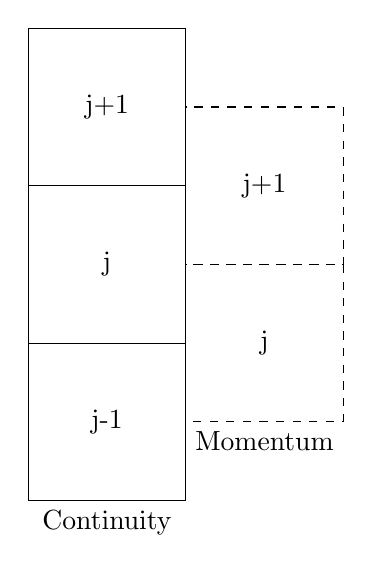
\begin{tikzpicture}
\draw (-2,-3) rectangle +(2,2);
\node[anchor=center] at (-1,-2) {j-1};
\draw (-2,-1) rectangle +(2,2);
\node[anchor=center] at (-1, 0) {j};
\draw (-2, 1) rectangle +(2,2);
\node[anchor=center] at (-1, 2) {j+1};
\draw[dashed] (-0,-2) rectangle +(2,2);
\node[anchor=center] at (1, -1) {j};
\draw[dashed] (-0, 0) rectangle +(2,2);
\node[anchor=center] at (1, 1) {j+1};
\node[anchor=north] at (-1, -3) {Continuity};
\node[anchor=north] at (1, -2) {Momentum};
\end{tikzpicture}
\end{center}
\caption{Illustration of indexing scheme.}
\label{fig:vertical_pipe_with_cells}
\end{figure}

Recalling the staggered grid from \sect{sect:topology}, the six scalar conservation laws, \eqref{eqn:conservation_of_ncg} -- \eqref{eqn:con_energy_liq}, are each integrated over the continuity volumes.
The assumption in these integrals is that the value of the conserved quantities and all thermodynamically-related variables are constant within a given volume.
\fig{fig:constant_value} shows a graphical representation of this idea for a generic function $f(x)$ over several spatial continuity meshes. For illustrative purposes, \eqref{eqn:conservation_of_liq} will be integrated over a given volume, $V_j$, as shown in \fig{fig:single_volume}.


\begin{figure}[ht]
\begin{center}
\includegraphics[width=0.5\textwidth]{images/constant_value.eps}
\end{center}
\caption{Constant variable values within computational volumes.}
\label{fig:constant_value}
\end{figure}


\begin{figure}[h!t]
\begin{center}
\includegraphics[width=0.5\textwidth]{images/single_volume.eps}
\end{center}
\caption{Single volume over which integration is done.}
\label{fig:single_volume}
\end{figure}

Within a given channel, $C_k$, a given continuity volume has a constant cross-sectional area, $A_{c_{j}}$, and a length of $\Delta x_{j}$.
The cross-sectional area of the boundary between two continuity volumes is given by the cross-section area of the momentum volume at that boundary, $A_{m}$.
The volume integrated equation is given by \eqref{eqn:spatially_discrete_liq_m_con}.

For the mass-flux terms evaluated on the continuity volume edge, the advected quantity is evaluated using a 1st order upwind method \cite{Tannehill1997}.
The velocity and cross-sectional area utilized in the continuity flux terms, $u_j$ and $A_{m,j}$, have the values defined at the center of the momentum volume that aligns with the edge of continuity volumes.
The sign of the velocity at the volume boundary determines the value of the donored quantity, $<a>_{d,j-\frac{1}{2}}$.
A generic formulation for this scheme is given by \eqref{eqn:upwind_donoring}.
The same general procedure is used for the other five scalar conservation equations.

\begin{IEEEeqnarray}{lcl}
\int_{V_j}\frac{\partial \left(\alpha_l \rho_l \right)}{\partial t } & + & \nabla \cdot \left( \alpha_l \rho_l u_l \right) \mathrm{d}V = \int_{V_j} \left(-(1-\eta)\Gamma^{'''} - S^{'''} + s_{m,l}\right) \mathrm{d}V \nonumber \\
V_j \frac{\partial \left(\alpha_{l,j} \rho_{l,j} \right)}{\partial t } & = & -\int_{V_j}\nabla \cdot \left( \alpha_l \rho_l u_l \right) \mathrm{d}V -(1-\eta_j)\Gamma_j - S_j + s_{m,l,j}V_j \nonumber \\
V_j \frac{\partial \left(\alpha_{l,j} \rho_{l,j} \right)}{\partial t } & = & -A_{m,j}\left[\alpha_l \rho_l u_l \right]_{x_{j-\frac{1}{2}}}^{x_{j+\frac{1}{2}}} -(1-\eta_j)\Gamma_j - S_j + s_{m,l,j}V_j \nonumber \\
\label{eqn:spatially_discrete_liq_m_con}
V_j \frac{\partial \left(\alpha_{l,j} \rho_{l,j} \right)}{\partial t } & = & -A_{m,j}\left( <\alpha_l \rho_l>_{d,j+\frac{1}{2}} u_{l,j+1} - <\alpha_l \rho_l>_{d,j-\frac{1}{2}} u_{l,j} \right) \nonumber \\
& & -(1-\eta)\Gamma_j - S_j + s_{m,l,j}V_j
\end{IEEEeqnarray}



\begin{equation}
\label{eqn:upwind_donoring}
<a>_{d, j-\frac{1}{2}} = \begin{cases} a_{j-1} &  u_j \geq 0 \\ a_{j} & u_j < 0 \end{cases}
\end{equation}

The three momentum conservation laws, \eqref{eqn:con_mom_liq} -- \eqref{eqn:con_mom_ent}, are integrated over their momentum volume.
The cross-sectional area for a momentum volume, $A_{m,j}$, can be defined independently of the two cross-sectional areas of the adjoining continuity volumes.
The momentum flux terms, \eqref{eqn:momentum_flux_terms}, are treated similarly to the flux terms in the continuity equations.
\begin{equation}
\label{eqn:momentum_flux_terms}
-\min\left(A_{m,j}, A_{m,j+1}\right)\left[<\alpha_l \rho_l u_l>_{d} u_l\right]_{x_{j-\frac{1}{2}}}^{x_{j+\frac{1}{2}}}
\end{equation}
There are two primary differences.
First, the momentum area is taken as the minimum of two adjoining momentum volumes.
Second, the velocity that is used to determine the origination of the donored quantity is the arithmetic mean of the velocities from the two adjacent momentum volumes, \eqref{eqn:average_advecting_vel}.

\begin{equation}
\label{eqn:average_advecting_vel}
u_{k,j+\frac{1}{2}} = \frac{1}{2}\left(u_{k,j} + u_{k, j+1}\right)
\end{equation}

The ordering of the governing equations within a continuity volumes is as follows:

\begin{enumerate}
\item{Conservation of \ncg{} field mass.}
\item{Conservation of vapor field mass.}
\item{Conservation of gaseous phase energy.}
\item{Conservation of liquid phase energy.}
\item{Conservation of entrained liquid field mass.}
\item{Conservation of continuous liquid field mass.}
\end{enumerate}

The conservation of momentum equations within a given momentum volume are ordered as follows:

\begin{enumerate}
\item{Conservation of continuous liquid field momentum.}
\item{Conservation of gaseous phase momentum.}
\item{Conservation of entrained liquid field momentum.}
\end{enumerate}

\subsection{Temporal Approximations}
\label{subsect:temporal_approx}

Once the governing conservation equations have been spatially discretized utilizing the method outlined above, the temporal derivatives need to be numerically approximated.
Using the spatially discrete approximations defined in \sect{subsect:spatial_approx}, the temporally continuous differential equations, \eqref{eqn:conservation_equations}, are now semi-discrete approximations given by \eqref{eqn:temporal_semi_discrete}, where $\vec{G}$ now represents the spatially discrete version of $\vec{g}$.

\begin{equation}
\label{eqn:temporal_semi_discrete}
\frac{\partial \,\vec{y} }{\partial t} = \vec{G}(\vec{y}(t))
\end{equation}

Given that there are nine conservation equations, the choice of which nine variables are the independent parameters which will be solved for is another distinguishing characteristic of safety analysis codes.
\cobra{} uses the following set of nine independent variables \eqref{eqn:independent_variables}.

\begin{equation}
\label{eqn:independent_variables}
\vec{x} = [\alpha_{ncg}P_{ncg}, \alpha_g, P, \alpha_e, \alpha_gS h_v, (1 - \alpha_g) h_l, \dot{m}_g, \dot{m}_l, \dot{m}_e]^{T}
\end{equation}

The definition of $\dot{m}_k$ is given by \eqref{eqn:mom_dot}.

\begin{equation}
\label{eqn:mom_dot}
\dot{m}_k = \alpha_k \rho_k u_k A_m
\end{equation}

Variants of these parameters include the use of velocities instead of momenta, temperatures or internal energies instead of enthalpies \cite{RELAP, TRACE}.

A distinguishing feature of the numerical method in \cobra{} is its treatment of the temporal derivative for the conservation of momentum.
In the work that follows, the temporal derivative of the conserved momentum equations is directly discretized, known as conservative form.
The other option, the non-conservative form, is to analytically expand the temporal derivative via the chain rule, \eqref{eqn:non_conservative}, and these equations are then temporally discretized.

\begin{equation}
\label{eqn:non_conservative}
\frac{\partial \alpha_k \rho_k u_k}{\partial t} = \alpha_k \rho_k \frac{\partial u_k}{\partial t} + u_k \frac{\partial \alpha_k \rho_k}{\partial t}
\end{equation}

Within \cobra{}, the temporal derivative is approximated by a one-step difference scheme, \eqref{eqn:simple_partial_t}, where the continuous time variables are now evaluated at discrete points, $t^0, t^1, \ldots, t^N$.
The notations $t^0$ and $t^N$ represents the initial and final time, respectively.
The term one-step refers to the fact that the temporal derivative involves only two consecutive points in time.

\begin{IEEEeqnarray}{rcl}
\int^{t^{n+1}}_{t^n}\frac{\partial \vec{y}(\vec{x})}{\partial t}\mathrm{d}\tau & = & \int^{t^{n+1}}_{t^n}\vec{G}(\vec{y}(\vec{x}))\mathrm{d}\tau \nonumber \\
\vec{y}(\vec{x}^{n+1}) - \vec{y}(\vec{x}^{n}) & = & \int_{t^{n+1}}^{t^n}\vec{G}(\vec{y}(\vec{x}))\mathrm{d}\tau \nonumber  \\
\frac{\vec{y}(\vec{x}^{n+1}) - \vec{y}(\vec{x}^{n})}{\int_{t^{n}}^{t^{n+1}}\mathrm{d} \tau} & = & \frac{\int_{t^{n+1}}^{t^n}\vec{G}(\vec{y}(\vec{x}))\mathrm{d}\tau}{\int_{t^{n}}^{t^{n+1}}\mathrm{d} \tau} \nonumber \\
\frac{\vec{y}(\vec{x}^{n+1}) - \vec{y}(\vec{x}^{n})}{\Delta t} & = & \frac{\int_{t^{n+1}}^{t^n}\vec{G}(\vec{y}(\vec{x}))\mathrm{d}\tau}{\int_{t^{n}}^{t^{n+1}}\mathrm{d} \tau} \nonumber \\
\label{eqn:simple_partial_t}
\frac{\vec{y}(\vec{x}^{n+1}) - \vec{y}(\vec{x}^{n})}{\Delta t} & = & \vec{G}(\vec{y}(\vec{x}^{*}))
\end{IEEEeqnarray}

The choice of how to approximate the temporal-average, $\vec{G}(\vec{y}(\vec{x}^{*}))$, hereafter referred to as $\vec{G}^{*}$, is a factor that defines the eventual solution algorithm.
There are two subcategories for solving this one-step temporal-integration problem, single-stage and multi-stage \cite{Stewart1981,LeVeque2007}.
\alg{alg:single_stage_temporal} shows how a multi-stage temporal integration scheme would work.

\begin{algo}[H]
\caption{Multi-stage temporal integration scheme.}
\label{alg:single_stage_temporal}
\setlength{\baselineskip}{0.625\baselineskip}
\begin{algorithmic}[1]
\Require $\vec{y}^{0}$ and $t^{0}$
\Set $n = 0$
\Loop \; Transient Loop
    \State $t^{n+1} : = t^{n} + \Delta t$
    \For{$j = 1 \to J$} \; Stage Loop
		\BlackBox Solve $\displaystyle \frac{\vec{y}^{j} - \vec{y}^{n}}{\Delta t} =  \vec{G}_{j}^{*}$ for $\vec{y}^{j}$.
	\EndFor
	\State $n = n + 1$
\EndLoop
\end{algorithmic}
\end{algo}

The final-stage conserved variables will be the new-time variables, $\vec{y}^{J} = \vec{y}^{n+1}$. 
At each stage the choice of how to approximate the driving function, $\vec{G}_{j}^{*}$, can change in both its functional dependence upon the stage values of $\vec{y}^{j}$ and in which components of $\vec{G}^{*}$ are included.
By excluding certain portions of $\vec{G}^{*}$ at certain stages, a time-splitting algorithm is developed.
By changing the functional dependencies of terms within $\vec{G}^{*}$ at different stages, predictor-corrector methods, also called stabilizing correction methods, are generated. 
A single-stage method is the degenerate case of $J = 1$.

The conserved quantities within a continuity volume are nonlinear functions of the chosen independent parameters, \eqref{eqn:nonlinear_functions}, regardless of the approximation chosen for $\vec{G}^{*}$.

\begin{equation}
\label{eqn:nonlinear_functions}
\vec{y}^{n+1} = \vec{y}(\vec{x}^{n+1})
\end{equation}

This nonlinearity necessitates the use of a nonlinear solver at every time-step.
Any dependence of $\vec{G}^{*}$ on the new time parameters can create additional nonlinearities.
The semi-discrete formulation, \eqref{eqn:simple_partial_t}, is expressed as a nonlinear function of $\vec{x}$ by \eqref{eqn:nonlinear_residuals}.

\begin{equation}
\label{eqn:nonlinear_residuals}
\vec{F}(\vec{x}^{n+1}) = \vec{y}(\vec{x}^{n+1}) - \vec{y}(\vec{x}^n) -\Delta t \vec{G}^{*}
\end{equation}

Depending upon the approximation of $\vec{G}^{*}$ and the number of stage, the temporal integration method used has an associated temporal accuracy.
The temporal accuracy is a way of quantifying the behavior of the solution as the time-step is reduced.
Order of accuracy estimates for temporal integration techniques are proportionality statements between the numerical error and a power of the time-step, $\mathcal{O}(\Delta t^k)$ \cite{LeVeque2007}. 
However, it has been shown that if the nonlinear problem, \eqref{eqn:nonlinear_residuals}, is not solved at every time step, the temporal accuracy of a method can be degraded \cite{Knoll2001, Mahaffy1993}.

\subsection{Nonlinear Approximations}
\label{subsect:nonlinear_approximations}

The method used to solve \eqref{eqn:nonlinear_residuals} for $\vec{x}^{n+1}$ in this work is Newton's method \cite{Deuflhard2004, Dennis1996}.
The nonlinear residual being solved is a function of the new-time unknowns, $\vec{x}^{n+1}$.
Newton's method is an iterative procedure to obtain $\vec{x}^{*}$ such that $\vec{F}(\vec{x}^{*}) = 0$.
Since Newton's method is an iterative procedure for obtaining new-time variables, two superscripts will be required.
The nonlinear iterate superscript will be $k$.
This iteration is done by successive linearization of the nonlinear problem \eqref{eqn:newton_taylor}, where $\vec{\delta x}^k = \vec{x}^{n+1,k+1} - \vec{x}^{n+1,k}$.

\begin{IEEEeqnarray}{rcccl}
0 & = & \vec{F}(\vec{x}^{n+1,k}+\vec{\delta x}^k) & = & \vec{F}(\vec{x}^{n+1,k}) +  \int_{\vec{x}^{n+1,k}}^{\vec{x}^{n+1,k}+\vec{\delta x}^k}\frac{\partial \vec{F}}{\partial \vec{x}}(\vec{z}) \mathrm{d} \vec{z} \nonumber \\
\label{eqn:newton_taylor}
0 & = & \vec{F}(\vec{x}^{n+1,k}+\vec{\delta x}^k) & \approx & \vec{F}(\vec{x}^{n+1,k}) + \vec{J}(\vec{x}^{n+1,k}) \cdot \vec{\delta x}^k
\end{IEEEeqnarray}

The algorithm is then one of finding successive updates, $\vec{\delta x}^k$, by solving \eqref{eqn:newton}.

\begin{equation}
\label{eqn:newton}
\vec{J}(\vec{x}^{n+1,k})\cdot \vec{\delta x}^k = -\vec{F}(\vec{x^{n+1,k}})
\end{equation} 

Since the system of nonlinear equations being solved represents a transient simulation, the iterations at each time-step start with an initial guess for the new time variables that is equal to the old-time variables, $\vec{x}^{n+1,0} = \vec{x}^{n}$.
The underlying assumption of this initial value is that the independent parameters will not change greatly over a time-step, and the old-time variables will provide an initial vector that is within the radius of convergence of Newton's method.
\alg{alg:local_newton} provides an overview of a transient simulation using a local Newton's method for a single-stage temporal integration scheme.
The algorithm generalizes to a multi-stage method by enclosing the Newton loop within a stage loop.

\begin{algo}[H]
\caption{Local Newton's method for single-stage temporal integration.}
\label{alg:local_newton}
\setlength{\baselineskip}{0.625\baselineskip}
\begin{algorithmic}[1]
\Require $\vec{x}^{0}$ and $t^{0}$
\Set $n = 0$
\Loop \; Transient Loop
    \State $t^{n+1} : = t^{n} + \Delta t$
    \State $k = 0$
    \State $\vec{x}^{n+1,k} = \vec{x}^{n}$
    \Loop \; Newton Loop
		\Calculate $\vec{F}(\vec{x}^{n+1,k})$ and $\vec{J}(\vec{x}^{n+1,k})$
		\Calculate $\vec{\delta x}^k = - \vec{J}^{-1}\cdot\vec{F}$
		\BlackBox $\vec{x}^{n+1,k+1}$
		\State $k = k + 1$
		\BlackBox Loop Termination Criteria
	\EndLoop
	\State $n = n + 1$
\EndLoop
\end{algorithmic}
\end{algo}

In \alg{alg:local_newton}, there are two black box calculations: the calculation of the updated independent parameters, $\vec{x}^{n+1,k+1}$; and the calculation of the loop termination criteria.
In the case of the loop termination criteria being $k > 0$, the resultant method is labeled as a single-shot linearization.
The exact nature of those two black box calculations is method-dependent and the various options will be discussed later.
In multi-stage temporal integration methods, both the update method and the loop termination criteria may vary between stages. 

%--------------------------------------------------------------------------------------------------------------------------------------------------------------------
%--------------------------------------------------------------------------------------------------------------------------------------------------------------------
%--------------------------------------------------------------------------------------------------------------------------------------------------------------------
%--------------------------------------------------------------------------------------------------------------------------------------------------------------------
%--------------------------------------------------------------------------------------------------------------------------------------------------------------------
%--------------------------------------------------------------------------------------------------------------------------------------------------------------------
%--------------------------------------------------------------------------------------------------------------------------------------------------------------------
\section{Solution Methods}
\label{sect:solution_techniques}

\sect{sect:numeric_approximation} provided a framework for characterizing the different methods used in thermal-hydraulic safety codes. 
Each method can be defined by the manner in which the temporal integration is carried out and the manner in which the nonlinearities are resolved.
The methods described below form the core of available techniques that have been developed for two-phase safety analysis codes. 
While each of the following methods has may have many subtly varying algorithmic implementations that have appeared in safety analysis software, the algorithms detailed below are general enough to encompass these variants.

\subsection{Fully Explicit Method}
\label{subsect:numerics_explicit}
The least computationally expensive method on a per time-step basis for temporally integrating \eqref{eqn:simple_partial_t} is a single-stage fully explicit method.
In the fully explicit method, the driving function is approximated as $\vec{G}(\vec{x}^n)$.
The only nonlinearities in this method are those present in the temporal derivative.
The vector notation formulation for this method is given by \eqref{eqn:explicit}. 

\begin{equation}
\label{eqn:explicit}
\vec{F}(\vec{x}^{n+1}) = \vec{y}^{n+1} - \vec{y}^{n} - \Delta t \vec{G}(\vec{y}(\vec{x}^{n}))
\end{equation}

The algorithmic implementation is shown in \alg{algo:explicit}.
Note that the momentum conservation equations have the identity matrix, $\vec{I}$, for their temporal Jacobian.
The continuity equations temporal Jacobian is a 6x6 matrix with no inter-volume coupling terms.

\begin{algo}[H]
\caption{Single-stage, fully explicit, single-shot linearization technique.}
\label{algo:explicit}
\setlength{\baselineskip}{0.625\baselineskip}
\begin{algorithmic}[1]
\Require $\vec{x}^{0}$ and $t^{0}$
\Set $n = 0$
\Loop \; Take a Time Step
    \State $t^{n+1} : = t^{n} + \Delta t$
    \Calculate $\vec{F}(\vec{x}^n)$ and $\vec{J}(\vec{x}^n)$
    \Calculate $\vec{\delta x} = -\vec{J}^{-1}\vec{F}$
    \Calculate $\vec{x}^{n+1} = \vec{x}^{n} + \vec{\delta x}$ 
\EndLoop{\;$n = n+1$}
\end{algorithmic}
\end{algo}

While this particular method is the least computationally expensive on a per time-step basis, it has a severe weakness.
That weakness is the Courant-Friedrichs-Lewy (CFL) limit imposed upon the time step size, $\Delta t$.
The CFL limit is a relationship between the spatial and temporal discretization and the characteristic velocities of information propagation in the problem of interest \cite{LeVeque2007, Tannehill1997}.
For the case of \eqref{eqn:explicit}, the CFL limit is given in \eqref{eqn:cfl_explicit}.

\begin{equation}
\label{eqn:cfl_explicit}
\Delta t_j \lesssim \frac{\Delta x_j}{|u_j|+|c_j|}
\end{equation}

Where $c_j$ is the speed of sound and $u_j$ is the magnitude of a given phasic velocity at a given location within the domain.
$\Delta t_j$ is calculated at every point within the domain using the known local fluid conditions.
The $\Delta t$ chosen for the $t^{n} \rightarrow t^{n+1}$ time-step is the most restrictive value over the domain.
While the explicit method may provide for the least computational cost on a per-time-step basis, the number of time-steps required for a given problem will be much higher due to the restrictive CFL limitations.

\begin{equation}
\label{eqn:global_cfl}
\Delta t = \min_{j \in \Omega} \Delta t_j
\end{equation}

Stated in words, the maximum permissible time-step size is determined by the most restrictive CFL limit within the domain which is limited by the local speed of sound, referred to as the sonic Courant limit.
This limitation of the explicit method prompted the development of alternative methods that were capable of exceeding this Courant limit.

\subsection{Fully Implicit Method}
\label{subsect:numerics_fully_implicit}
An alternative method for integrating \eqref{eqn:temporal_semi_discrete} is to use a fully implicit discretization of $\vec{G}^{*}$ \cite{Frepoli2003, Barre1990}.
The fully implicit method temporally approximates $\vec{G}^{*}$ as a function only of new-time parameters, \eqref{eqn:implicit}.

\begin{equation}
\label{eqn:implicit}
\vec{F}(\vec{x}^{n+1}) = \vec{y}^{n+1} - \vec{y}^{n} - \Delta t \vec{G}(\vec{y}(\vec{x}^{n+1}))
\end{equation}

This method has the advantage of not being limited by a CFL number for stability purposes; it is unconditionally stable.
However, the solution of \eqref{eqn:implicit} is the most computationally expensive on a per time-step basis of the methods considered.
The computational implementation of a fully implicit method is presented in \alg{algo:implicit}.

\begin{algo}[H]
\setlength{\baselineskip}{0.625\baselineskip}
\begin{algorithmic}[1]
\Require $\vec{x}^{0}$ and $t^{0}$
\Set $n = 0$
\Loop \; Transient Loop
    \State $t^{n+1} : = t^{n} + \Delta t$
    \For{$j = 1 \to 2$} \; Stage Loop
    \State $k = 0$
    \State $\vec{x}^{k} = \vec{x}^{n}$
    \Loop \; Newton Loop
		\Calculate $\vec{F}(\vec{x}^{k})$ and $\vec{J}(\vec{x}^{k})$
		\Calculate $\vec{\delta x}^k = - \vec{J}^{-1}\cdot\vec{F}$
		\BlackBox $\vec{x}^{k+1}$
		\State $k = k + 1$
		\BlackBox Loop Termination Criteria
	\EndLoop	
	\EndFor
	\State $n = n + 1$
\EndLoop
\end{algorithmic}
\caption{Fully implicit, two-stage, nonlinear solver method.}
\label{algo:implicit}
\end{algo}

\subsection{Semi-Implicit Method}
\label{subsect:semi_implicit}

The semi-implicit method was developed to overcome the sonic Courant limitations of the explicit method while avoiding the computational cost of the fully implicit method \cite{Liles1978}.
Since the work being done here will deal with the semi-implicit method, detailed description of the semi-implicit equations used in \cobra{} are provided.
The momentum equations, neglecting spatial discretization notation and external sources, are given in \eqref{eqn:si_mom_liq} -- \eqref{eqn:si_mom_ent}.

\begin{IEEEeqnarray}{rCl}
\label{eqn:si_mom_liq}
\dot{m}_{l}^{n+1} - \dot{m}_{l}^{n} & = & \frac{\Delta t}{\Delta x}\left(- \sum_{NK} \left( (\alpha_l \rho_l u_l) u_l \cdot \vec{\bar{n}}\right)^{n}
 -\alpha^{n}_l \nabla P^{n+1} + (\alpha_l \rho_l)^{n} g - K^{n}_{wl}(\dot{m}_l^{n+1})^2 \right. \nonumber \\
 & + & \left. K^{n}_{i,gl}(\dot{m}^{n+1}_l - \dot{m}_g^{n+1})^2 - ((1 - \eta)\Gamma u^{'})^{n} - (S u^{'})^{n}\vphantom{\sum_{NK}}\right) \\
\label{eqn:si_mom_gas}
\dot{m}_{g}^{n+1} - \dot{m}_{g}^{n} & = & \frac{\Delta t}{\Delta x}\left(- \sum_{NK} \left( (\alpha_g \rho_g u_g) u_g  \cdot \vec{\bar{n}}\right)^{n}  -\alpha^{n}_g \nabla P^{n+1} + (\alpha_g \rho_g)^{n} g - K^{n}_{wg}(\dot{m}_g^{n+1})^2 \right.\nonumber \\
& - & \left. K^{n}_{i,gl}(\dot{m}^{n+1}_l - \dot{m}_g^{n+1})^2 -K^{n}_{i,ge}(\dot{m}^{n+1}_e - \dot{m}_g^{n+1})^2 + (\Gamma u^{'})^{n}\vphantom{\sum_{NK}}\right) \\
\label{eqn:si_mom_ent}
\dot{m}_{e}^{n+1} - \dot{m}_{e}^{n} & = & \frac{\Delta t}{\Delta x}\left(- \sum_{NK} \left( (\alpha_e \rho_l u_e) u_e  \cdot \vec{\bar{n}}\right)^n -\alpha^{n}_e \nabla P^{n+1} + (\alpha_e \rho_l)^{n} g - K^{n}_{we}(\dot{m}_e^{n+1})^2\right. \nonumber \\
&+& \left. K^{n}_{i,ge}(\dot{m}^{n+1}_e - \dot{m}_g^{n+1})^2 - (\eta \Gamma u^{'})^{n} + (S u^{'})^n\vphantom{\sum_{NK}}\right)
\end{IEEEeqnarray}

In the above equations, the flux terms are summed over $NK$, which indicates the number of continuity volumes connected to a given momentum volume.
The coefficients $K$ represent effective friction factors calculated using parameters only from time n.
The interfacial transfer terms are explicitly evaluated.
The only new time parameters used in \eqref{eqn:si_mom_liq} -- \eqref{eqn:si_mom_ent} are flow rates and pressures.
The purely explicit evaluation of the momentum advection term is what leads to a CFL limits known as the material Courant limit.
Similar to the sonic Courant limit discussed in \sect{subsect:numerics_explicit}, the material Courant limit dictates the largest $\Delta t$ that can be achieved while maintaining a stable solution algorithm.
In this method, the Courant limit is given by \eqref{eqn:si_cfl}.
The characteristic velocity is now a phasic velocity only.
This allows for much greater time-step sizes than the explicit method, but it is still limited.

\begin{equation}
\label{eqn:si_cfl}
\Delta t_j \lesssim \frac{\Delta x_j}{|u_{k,j}|}
\end{equation}

The continuity equations used in this work, omitting external sources, are shown in \eqref{eqn:si_mass_ncg} -- \eqref{eqn:si_nrg_liq}.

\begin{IEEEeqnarray}{rCl}
\label{eqn:si_mass_ncg}
V_c (\alpha_g \rho_{n})^{n+1} & - & V_c (\alpha_g \rho_{n})^{n} = -\Delta t \sum_{NK}\left( <\alpha^{n}_g \rho^{n}_{n}>^{n}_{d} u^{n+1}_g  \cdot \vec{\bar{n}}\right) \\
\label{eqn:si_mass_vap}
V_c \left(\alpha_g \rho_v \right)^{n+1} &-& V_c \left(\alpha_g \rho_v \right)^{n} = - \Delta t \sum_{NK} \left( <\alpha^{n}_g \rho^{n}_v>^{n}_{d} u^{n+1}_g  \cdot \vec{\bar{n}}\right) + \Delta t \Gamma^{n+1} \\
\label{eqn:si_mass_liq}
V_c \left(\alpha_l \rho_l \right)^{n+1} & - & V_c \left(\alpha_l \rho_l \right)^{n} =  -\Delta t \sum_{NK}\left( <\alpha^n_l \rho^n_l>^{n}_{d} u^{n+1}_l  \cdot \vec{\bar{n}}\right) \nonumber \\
&- &\Delta t\left[(1-\eta)\Gamma + S \right]^{n+1} \\
\label{eqn:si_mass_ent}
V_c \left(\alpha_e \rho_l \right)^{n+1} & - & V_c \left(\alpha_e \rho_l \right)^{n} = -\Delta t \sum_{NK}\left( <\alpha^{n}_e \rho^{n}_l>^{n}_{d} u^{n+1}_e  \cdot \vec{\bar{n}}\right)\nonumber \\ 
&+& \Delta t\left[ S -\eta\Gamma \right]^{n+1} \\
\label{eqn:si_nrg_gas}
V_c \left( \alpha_g \{\rho_g h_g\} \right)^{n+1} & - & V_c \left( \alpha_g \{\rho_g h_g\} \right)^{n}  = -\Delta t \sum_{NK} \left(  <\alpha^{n}_g \{\rho_g h_g\}^{n}>^{n}_{d} u^{n+1}_g  \cdot \vec{\bar{n}}\right) \nonumber \\
&+& \Delta t \left[\Gamma h^{'}_v + q_{i,v} + q_{gl} + q_{wg} \right]^{n+1} + V_c \alpha^{n}_g ( P^{n+1} - P^{n} ) \\
\label{eqn:si_nrg_liq}
V_c\left( \alpha_l \rho_l h_l \right)^{n+1} & - & V_c\left( \alpha_l \rho_l h_l \right)^{n} =  -\Delta t \sum_{NK} \left( <\alpha^{n}_l \rho^{n}_l h^{n}_l>^{n}_{d} u^{n+1}_l \cdot \vec{\bar{n}} + <\alpha^{n}_e \rho^{n}_l h^{n}_l>^{n}_{d} u^{n+1}_e  \cdot \vec{\bar{n}}\right) \nonumber \\
& +& \Delta t \left[q_{wl} -\Gamma h^{'}_l +  q_{i,l} - q_{gl}\right]^{n+1} + V_c \alpha^{n}_l (P^{n+1} - P^{n})
\end{IEEEeqnarray}

The flux terms include new time velocities, $u^{n+1}_k$.
Since \cobra{} uses $\dot{m}_{k}$ as independent parameters, the velocities are derived quantities, whose functional form is given in \eqref{eqn:si_vel}.
The $<\alpha_k \rho_k>^{n}_{a}$ represents the arithmatic average of macroscopic densities from adjoining continuity volumes.

\begin{equation}
\label{eqn:si_vel}
u^{n+1}_k = \frac{\dot{m}^{n+1}_k}{A_m <\alpha_k \rho_k>^{n}_{a}} 
\end{equation}

The donoring operator $<a^n>^{n}_{d}$ is an extension of \eqref{eqn:upwind_donoring}.
The donored quantities and the velocity used to determine the direction of donoring are evaluated with their old-time values.

\cobra{} uses a single-shot linearization method to resolve the nonlinearities.
\alg{alg:si_legacy} shows the traditional algorithm.
Due to the nature of the semi-implicit method, step 5 of \alg{alg:si_legacy} requires additional details.
The linear algebra problem to be solved during step 5 is presented in \eqref{eqn:si_solve} for a simply connected problem with three continuity volumes and three momentum volumes.

\begin{algo}[H]
\caption{\cobra{} semi-implicit solution algorithm}
\label{alg:si_legacy}
\setlength{\baselineskip}{0.625\baselineskip}
\begin{algorithmic}[1]
\Require $\vec{x}^{0}$ and $t^{0}$
\Set $n = 0$
\Loop \; Transient Loop
    \State $t^{n+1} : = t^{n} + \Delta t$
	\Calculate $\vec{F}(\vec{x}^{n})$ and $\vec{J}(\vec{x}^{n})$
	\BlackBox $\vec{\delta x} = - \vec{J}^{-1}\cdot\vec{F}$
	\Calculate $\vec{x}^{n+1} = \vec{x}^{n} + \vec{\delta x}$
	\State $n = n + 1$
\EndLoop
\end{algorithmic}
\end{algo}


 \begin{equation}
 \label{eqn:si_solve}
 \begin{bmatrix} 
 \vec{J}_{m_1,m_1} & \vec{J}_{m_1,c_1} & \vec{0} & \vec{0} & \vec{0} & \vec{0}\\
 \vec{J}_{c_1,m_1} & \vec{J}_{c_1,c_1} & \vec{J}_{c_1,m_2} & \vec{0} & \vec{0} & \vec{0} \\
 \vec{0} & \vec{J}_{m_2,c_1} & \vec{J}_{m_2,m_2} & \vec{J}_{m_2,c_2} & \vec{0} & \vec{0} \\
 \vec{0} & \vec{0} & \vec{J}_{c_2,m_2} & \vec{J}_{c_2,c_2} & \vec{J}_{c_2,m_3} & \vec{0} \\
 \vec{0} & \vec{0} & \vec{0} & \vec{J}_{m_3,c_2} & \vec{J}_{m_3,m_3} & \vec{J}_{m_3,c_3} \\ 
 \vec{0} & \vec{0} & \vec{0} & \vec{0} & \vec{J}_{c_3,m_3} & \vec{J}_{c_3,c_3}  
 \end{bmatrix} \begin{bmatrix}
 \vec{\delta m}_{1} \\ \vec{\delta c}_{1} \\
 \vec{\delta m}_{2} \\ \vec{\delta c}_{2} \\
 \vec{\delta m}_{3} \\ \vec{\delta c}_{3}
\end{bmatrix}  = -\begin{bmatrix}
 \vec{F}_{m_1} \\ \vec{F}_{c_1} \\
 \vec{F}_{m_2} \\ \vec{F}_{c_2} \\
 \vec{F}_{m_3} \\ \vec{F}_{c_3} \end{bmatrix}
 \end{equation}
 
 The semi-implicit solution framework is composed of five steps.
 First, the momentum volume equations, rows one, three, and five of the linear system \eqref{eqn:si_solve}, are multiplied by their inverse diagonal Jacobian entries, $\vec{J}_{m_k}$.
 The off-diagonal entries for the momentum equations are now $\vec{J}^{-1}_{m_k}\vec{J}_{m_k,c_j}$ where $j$ is the index of the connected continuity volumes.
 Since the $J_{m_k,c_j}$ terms only contain derivatives with respect to the pressure for the adjoining continuity volumes, the product $\vec{J}^{-1}_{m_k}\vec{J}_{m_k,c_j}$ will be referred to as $\frac{\partial \vec{m}_k}{\partial P_j}$.
 Using the above notation, the resulting system is given in \eqref{eqn:si_solve_1}.
 
  \begin{equation}
 \label{eqn:si_solve_1}
 \begin{bmatrix} 
 \vec{I} & \frac{\partial \vec{m}_1}{\partial P_1} & \vec{0} & \vec{0} & \vec{0} & \vec{0}\\
 \vec{J}_{c_1,m_1} & \vec{J}_{c_1} & \vec{J}_{c_1,m_2} & \vec{0} & \vec{0} & \vec{0} \\
 \vec{0} & \frac{\partial \vec{m}_2}{\partial P_1} & \vec{I} & \frac{\partial \vec{m}_2}{\partial P_2} & \vec{0} & \vec{0} \\
 \vec{0} & \vec{0} & \vec{J}_{c_2,m_2} & \vec{J}_{c_2} & \vec{J}_{c_2,m_3} & \vec{0} \\
 \vec{0} & \vec{0} & \vec{0} & \frac{\partial \vec{m}_{3}}{\partial P_2} & \vec{I} & \frac{\partial \vec{m}_{3}}{\partial P_3} \\ 
 \vec{0} & \vec{0} & \vec{0} & \vec{0} & \vec{J}_{c_3,m_3} & \vec{J}_{c_3}  
 \end{bmatrix} \begin{bmatrix}
 \vec{\delta m}_{1} \\ \vec{\delta c}_{1} \\
 \vec{\delta m}_{2} \\ \vec{\delta c}_{2} \\
 \vec{\delta m}_{3} \\ \vec{\delta c}_{3}
\end{bmatrix}  = -\begin{bmatrix}
 \vec{J}^{-1}_{m_1}\vec{F}_{m_1} \\ \vec{F}_{c_1} \\
 \vec{J}^{-1}_{m_2}\vec{F}_{m_2} \\ \vec{F}_{c_2} \\
 \vec{J}^{-1}_{m_3}\vec{F}_{m_3} \\ \vec{F}_{c_3} \end{bmatrix}
 \end{equation}

Second, the momentum equations are used to eliminate the $\vec{J}_{c_k,m_k}$ entries from the continuity volumes.
The resulting equation set no longer has equations for the momentum volumes, \eqref{eqn:si_solve_2}.

\begin{IEEEeqnarray}{rl}
\label{eqn:si_solve_2}
\begin{bmatrix} 
\vec{J}_{c_1} - \vec{J}_{c_1,m_1}\frac{\partial \vec{m}_1}{\partial P_1} - \vec{J}_{c_1,m_2}\frac{\partial \vec{m}_2}{\partial P_1} &
-\vec{J}_{c_1,m_2}\frac{\partial \vec{m}_2}{\partial P_2} &
\vec{0} \\
-\vec{J}_{c_2,m_2}\frac{\partial \vec{m}_2}{\partial P_1} & 
\vec{J}_{c_2} - \vec{J}_{c_2,m_2}\frac{\partial \vec{m}_2}{\partial P_2}-\vec{J}_{c_2,m_3}\frac{\partial \vec{m}_3}{\partial P_2} &
-\vec{J}_{c_2,m_3}\frac{\partial \vec{m}_3}{\partial P_3} \\
 \vec{0} &
-\vec{J}_{c_3,m_3}\frac{\partial \vec{m}_3}{\partial P_2} &
\vec{J}_{c_3} -\vec{J}_{c_3,m_3}\frac{\partial \vec{m}_3}{\partial P_3} 
\end{bmatrix} &\begin{bmatrix}
\vec{\delta c}_{1} \\
\vec{\delta c}_{2} \\
\vec{\delta c}_{3}
\end{bmatrix} \nonumber \\
 = -\begin{bmatrix}
\vec{F}_{c_1} -
\vec{J}_{c_1,m_1}\vec{J}^{-1}_{m_1}\vec{F}_{m_1}-\vec{J}_{c_1,m_2}\vec{J}^{-1}_{m_2}\vec{F}_{m_2} \\
\vec{F}_{c_2} - 
\vec{J}_{c_2,m_2}\vec{J}^{-1}_{m_2}\vec{F}_{m_2}-\vec{J}_{c_2,m_3}\vec{J}^{-1}_{m_3}\vec{F}_{m_3} \\
\vec{F}_{c_3} - 
\vec{J}_{c_3,m_3}\vec{J}^{-1}_{m_3}\vec{F}_{m_3}
\end{bmatrix} &
 \end{IEEEeqnarray}

The off-diagonal entries of the reduced Jacobian matrix in \eqref{eqn:si_solve_2}, $\vec{J}_{c_i,m_j}\frac{\partial \vec{m}_j}{\partial P_k}$ will be denoted by $\vec{C}_{c_i,P_j}$ as they represent the change in the continuity variables in volume $i$ due to the change in the pressure of continuity volume $j$.
The $6 x 6$ matrix, $\vec{C}_{c_i,P_j}$, contains only entries in the last column, which correspond to the inter-continuity pressure coupling terms.
The diagonal entries of the reduced Jacobian and the right-hand side entries will be referred to as $\vec{J}^{*}_{c_i}$ and $\vec{F}^{*}_{c_i}$.
With the new nomenclature, \eqref{eqn:si_solve_2} can be restated as \eqref{eqn:si_solve_3}.

  \begin{equation}
 \label{eqn:si_solve_3}
 \begin{bmatrix} 
 \vec{J}^{*}_{c_1} & \vec{C}_{c_1,P_2} & \vec{0} \\
 \vec{C}_{c_2,P_1} & \vec{J}^{*}_{c_2} & \vec{C}_{c_2,P_3} \\
 \vec{0}           & \vec{C}_{c_3,P_2} & \vec{J}^{*}_{c_3}
 \end{bmatrix} \begin{bmatrix}
 \vec{\delta c}_{1} \\
 \vec{\delta c}_{2} \\
 \vec{\delta c}_{3}
\end{bmatrix}  = -\begin{bmatrix}
 \vec{F}^{*}_{c_1} \\
 \vec{F}^{*}_{c_2} \\
 \vec{F}^{*}_{c_3}
\end{bmatrix}
 \end{equation}

Step three is to multiply each row by the $\vec{L}^{-1}_{c_i}$ portion of the LU decomposition without pivoting of $\vec{J}^{*}_{c_i}$, \eqref{eqn:si_solve_4}

  \begin{equation}
 \label{eqn:si_solve_4}
 \begin{bmatrix} 
 \vec{U}^{*}_{c_1} & \vec{L}^{-1}_{c_1}\vec{C}_{c_1,P_2} & \vec{0} \\
 \vec{L}^{-1}_{c_2}\vec{C}_{c_2,P_1} & \vec{U}^{*}_{c_2} & \vec{L}^{-1}_{c_2}\vec{C}_{c_2,P_3} \\
 \vec{0}           & \vec{L}^{-1}_{c_3}\vec{C}_{c_3,P_2} & \vec{U}^{*}_{c_3}
 \end{bmatrix} \begin{bmatrix}
 \vec{\delta c}_{1} \\
 \vec{\delta c}_{2} \\
 \vec{\delta c}_{3}
\end{bmatrix}  = -\begin{bmatrix}
 \vec{L}^{-1}_{c_1}\vec{F}^{*}_{c_1} \\
 \vec{L}^{-1}_{c_2}\vec{F}^{*}_{c_2} \\
 \vec{L}^{-1}_{c_3}\vec{F}^{*}_{c_3}
\end{bmatrix}
 \end{equation}
 
By isolating the last row from each continuity block and dividing that row by its diagonal entry, a resulting matrix for the pressure update in every continuity volume is obtained, \eqref{eqn:si_pressure_matrix}. 
For a problem with $N$ continuity volumes, the resulting pressure matrix, \eqref{eqn:si_pressure_matrix}, will be $N$ x $N$.

  \begin{equation}
 \label{eqn:si_pressure_matrix}
 \begin{bmatrix} 
 1 & \frac{\vec{L}^{-1}_{c_1}\vec{C}_{c_1,P_2}[6]}{\vec{U}^{*}_{c_1}[6]} & \vec{0} \\
 \frac{\vec{L}^{-1}_{c_2}\vec{C}_{c_2,P_1}[6]}{\vec{U}^{*}_{c_2}[6]} & 1 & \frac{\vec{L}^{-1}_{c_2}\vec{C}_{c_2,P_3}[6]}{\vec{U}^{*}_{c_2}[6]} \\
 \vec{0}           & \frac{\vec{L}^{-1}_{c_3}\vec{C}_{c_3,P_2}[6]}{\vec{U}^{*}_{c_3}[6]} & 1
 \end{bmatrix} \begin{bmatrix}
 \vec{\delta P}_{1} \\
 \vec{\delta P}_{2} \\
 \vec{\delta P}_{3}
\end{bmatrix}  = -\begin{bmatrix}
 \frac{\vec{L}^{-1}_{c_1}\vec{F}^{*}_{c_1}[6]}{\vec{U}^{*}_{c_1}[6]} \\
 \frac{\vec{L}^{-1}_{c_2}\vec{F}^{*}_{c_2}[6]}{\vec{U}^{*}_{c_2}[6]} \\
 \frac{\vec{L}^{-1}_{c_3}\vec{F}^{*}_{c_3}[6]}{\vec{U}^{*}_{c_3}[6]}
\end{bmatrix}
 \end{equation}

In step four, the pressure matrix is then solved for the pressure updates in every continuity volume.
This step is performed using the sparse-matrix solver, SuperLU \cite{Li1999}. 

Step five is the use the vector of pressure updates to obtain the continuity updates in every volume from \eqref{eqn:si_solve_4} and to obtain the updates for the momentum variables from the momentum rows of \eqref{eqn:si_solve_1}.

This five step process provides an overview of the solution technique of the semi-implicit method used in \cobra{}.
As \cobra{} is a single-shot algorithm, no additional Newton steps would be taken.

\subsection{Stability-Enhancing Two-Step Method} 
\label{subsect:numerics_sets}
In order to overcome the material Courant limit placed upon the simulation by the semi-implicit method, the Stability Enhancing Two-Step (SETS) method was developed \cite{Mahaffy1982}.
While not unconditionally stable, as the fully implicit method, the SETS method allows for time-steps to exceed the material Courant limit.
The SETS method overcomes the material Courant limit by taking a multi-stage approach to the temporal integration.
The SETS method presented below uses velocities as independent parameters, not momenta.
While there are variants of the SETS method \cite{TRACE}, \alg{alg:sets} reflects the original publication.

There are three stages in the original SETS method.
Stage one is a single-shot linearized solution of the momentum equations where the velocity terms in the momentum equations of $\vec{G}^{*}$ are evaluated implicitly.
The lack of implicit dependence upon any continuity variables allows each volume to be solved independently.
This step results in predicted $u^{*}_{k}$ phasic velocities.
In stage two, the momentum and continuity equations are solved using a traditional semi-implicit scheme with two primary exceptions.
The first difference is that the momentum flux terms are evaluated using the stage-one predicted velocities as the advecting velocities.
The second difference is that the nonlinearities in the momementum equations, arising from interfacial and wall drag, are subject to a single-shot linearization.
The single-shot nature of the momentum equations allows for the reduction of the system into coupled continuity volumes as in the semi-implicit method.
The nonlinear continuity equations are then solved via Newton's method.
Stated another way, the Jacobians for the momentum equations are fixed at the first iterate, while the Jacobians for the mass and energy equations are updated at each iterate.
The only results from stage two that are used in stage three are the final velocities, $\vec{u}^{n+1}$.
Stage three, the mass and energy equations are solved such that all continuity variables are implicit and the final time velocities are from stage two.
The resulting system of coupled continuity equations is then solved.
For each stage, the residual and Jacobian matrix will be denoted by $\vec{F}_k$ and $\vec{J}_k$, with $k = 1 \to 3$.

\begin{algo}[H]
\caption{SETS Method}
\label{alg:sets}
\setlength{\baselineskip}{0.625\baselineskip}
\begin{algorithmic}[1]
\Require $\vec{x}^{0}$ and $t^{0}$
\Set $n = 0$
\Loop \; Transient Loop
    \State $t^{n+1} : = t^{n} + \Delta t$
	\Calculate $\vec{F}_1$ and $\vec{J}_1$
	\Calculate $\vec{u}^{*}$ from $\vec{\delta u}^{*} = -\vec{J}^{-1}_1\vec{F}_1$
	\Loop \; Newton Loop
		\Calculate $\vec{F}_2$ and $\vec{J}_2$
		\BlackBox $\vec{\delta x} = - \vec{J}_2^{-1}\vec{F}_2$
		\Calculate $\vec{x}^{n+1} = \vec{x}^{n} + \vec{\delta x}$
		\BlackBox Loop Termination Criteria
	\EndLoop
	\Calculate $\vec{x}^{n+1}$ from $\vec{F}_3$.
	\State $n = n + 1$
\EndLoop
\end{algorithmic}
\end{algo}

This algorithm allows for the semi-implicit method to be used within a larger framework.
The loop termination criteria is an implementation-specific choice.
The TRACE code uses an $L_{inf}$ norm of the unscaled Newton updates for the continuity variables to determine convergence.

\subsection{Nearly-Implicit Method}
\label{subsect:numerics_nearly_implicit}
Another possible method used to overcome the material Courant limit without incurring the same computational cost as the fully implicit method is the Nearly-Implicit method \cite{Trapp1986, RELAP}.

The Nearly-Implicit method is a multi-stage temporal integration scheme.
In the first stage, the approximation  of $\vec{G}^{*}$ is one in which the mass and energy terms are implicit except for the donored values in the flux terms. 
In addition, the the chain rule is applied to the continuous temporal derivatives, resulting in mass equations like \eqref{eqn:ni_dt}.
The energy temporal derivatives are similarly expanded.

\begin{equation}
\label{eqn:ni_dt}
\frac{\partial \alpha_k \rho_k}{\partial t} = \alpha_k \frac{\partial \rho_k}{\partial t} + \rho_k \frac{\partial \alpha_k}{\partial t}
\end{equation}

The temporal discretization of \eqref{eqn:ni_dt} is given by \eqref{eqn:ni_dis_dt}.

\begin{equation}
\label{eqn:ni_dis_dt}
\alpha_k \frac{\partial \rho_k}{\partial t} + \rho_k \frac{\partial \alpha_k}{\partial t} = \alpha^n_k\frac{ \rho^{n+1}_k - \rho^{n}_k}{\Delta t} + \rho^{n}_k\frac{\alpha^{n+1}_k} - \alpha^{n}_k{\Delta t}
\end{equation}

The momentum equations are implicit in all interfacial exchange terms, the pressure terms, and the momentum flux terms.

The Nearly-Implicit method is a three-stage solution process.
The first stage is similar to the semi-implicit method.
However, as opposed to the semi-implicit method, where the momentum variables are eliminated from the equations being solved, in the Nearly-Implicit method, it is the mass and energy equations that are used to eliminate the pressure terms from the momentum equations.
The resulting matrix is a linear system of coupled velocities.
The stage-one velocities are taken to be the new-time velocities.
Once the stage-one velocities are obtained, the corresponding stage-one continuity variables are obtained analogously to the new-time momentum in the semi-implicit method.
Stage one is a single-shot linearization.
In the second stage, only the continuity equations are solved and they are in conservative form.
The interfacial exchange terms in the mass and energy equations are evaluated using the stage-one continuity variables.
The resulting system of equations is linear in the conserved quantities.
This linear system is solved for the conserved quantities.
In stage three, the nonlinear relation between the conserved quantities and the independent parameters is then approximated via a single-shot linearization of the equations of state.
\alg{alg:ni} shows the three-stage process.

\begin{algo}[H]
\caption{Nearly-Implicit Method}
\label{alg:ni}
\setlength{\baselineskip}{0.625\baselineskip}
\begin{algorithmic}[1]
\Require $\vec{x}^{0}$ and $t^{0}$
\Set $n = 0$
\Loop \; Transient Loop
    \State $t^{n+1} : = t^{n} + \Delta t$
	\Calculate $\vec{F}_1$ and $\vec{J}_1$
	\Calculate $\vec{c}^{*}$ and $\vec{u}^{n+1}$ from $\vec{\delta x}^{*} = -\vec{J}^{-1}_1\vec{F}_1$
	\Calculate $\vec{F}_2$
	\Calculate $\vec{c}^{**}$ from $\vec{F}_2$
	\Calculate $\vec{c}^{n+1}$ from $\vec{F}_3$.
	\State $n = n + 1$
\EndLoop
\end{algorithmic}
\end{algo}


%--------------------------------------------------------------------------------------------------------------------------------------------------------------------
%--------------------------------------------------------------------------------------------------------------------------------------------------------------------
%--------------------------------------------------------------------------------------------------------------------------------------------------------------------
%--------------------------------------------------------------------------------------------------------------------------------------------------------------------
%--------------------------------------------------------------------------------------------------------------------------------------------------------------------
%--------------------------------------------------------------------------------------------------------------------------------------------------------------------
%--------------------------------------------------------------------------------------------------------------------------------------------------------------------
\section{Algorithmic Concerns}
\label{sect:algorithmic_concerns}

The methods outlined in \sect{sect:solution_techniques} have algorithmic issues that need to be addressed.
Given that the governing conservation laws in thermal-hydraulic analyses are those of two-phase flow, there is no systematic and widely agreed upon way of dealing with phase appearance or disappearance.
While each algorithmic implementation of the various methods addresses these issues out of necessity, there is no systematic, or optimal, way of doing so. 

Phase and field appearance or disappearance, hereafter referred to as phase transitions, is a concern for any algorithmic implementation of thermal hydraulic methods.
The methods for addressing phase transitions within two-phase analysis software are ad-hoc procedures that vary from software to software.
However, certain physical limits have been identified that need to be considered \cite{Bestion2000}.
Since the manner in which \cobra{} treats phase transitions is of importance to this work, a brief description will follow.

\begin{itemize}
\item{Velocity equilibrium enforced by enhanced interfacial drag.}
\item{Minimum field threshold for the three water fields.}
\item{Partial pressure of \ncg field allowed to go to zero.}
\end{itemize}

Within \cobra{}, there are certain constraints that are imposed upon the independent parameters.
These constraints are dealt with in a mitigative manner.
After a single Newton step, the updated parameters evaluated to determine their validity in the context of a single-shot method.
There are two ways of resolving potentially invalid solutions: limiting and failure.
The limiting procedure can either truncate the updated parameter, so that is falls within a valid range or the time-step can be considered a failure.
When a predicted volume fraction falls outside of its valid range, it is limited.
When thermodynamic variables are predicted to exceed the equations of state available in \cobra{}, the time-step is repeated with a smaller time-step size. 

There are also limits placed upon the changes in the continuity parameters.
\begin{itemize}
\item{Change of enthalpy too great.}
\item{Change in pressure too great.}
\item{Change in partial pressure of \ncg field too great.}
\end{itemize}

Another algorithmic concern is how to identify a potentially poor linearization point in the presence of phase transitions. 
This can be considered a predictive error correction technique.
It uses information from the explicit portion of the nonlinear residual to identify situations where the linearization point may be poor.
In \cobra{} this method is used only for the prediction of \ncg{} appearance.

%--------------------------------------------------------------------------------------------------------------------------------------------------------------------
%--------------------------------------------------------------------------------------------------------------------------------------------------------------------
%--------------------------------------------------------------------------------------------------------------------------------------------------------------------
%--------------------------------------------------------------------------------------------------------------------------------------------------------------------
%--------------------------------------------------------------------------------------------------------------------------------------------------------------------
%--------------------------------------------------------------------------------------------------------------------------------------------------------------------
%--------------------------------------------------------------------------------------------------------------------------------------------------------------------
\section{Domain Coupling}
\label{sect:code_coupling}

\cobra{} possesses the physics necessary to model the complicated flow patterns encountered during LOCA within the core of an NPP.
However, it lacks the detailed models for NPP components (steam-generators, heat exchanges, etc) that are traditionally available from system-analysis codes.
When modeling full NPP transients, it is advantageous to use sub-channel software for the core and system analysis software to model the rest of the NPP.
The combination of different specialized software is a common practice.
This coupling of capabilities can be accomplished in two ways: the two pieces of software can be merged, or they can be coupled via data exchange.
Examples of the first method are MARS \cite{Jeong2008} and TRACE \cite{TRACE}.
Coupling software via data exchange is the more common option \cite{Makihara2003, Aumiller2002, Aumiller2001, Avramova2006, Weaver2002}.

The use of explicit coupling can lead to a sonic Courant limit imposed upon the two coupled systems \cite{Ragusa2009, Aumiller2000}.
The coupling of software via data exchange has led to the development of a semi-implicit coupling technique for thermal-hydraulic simulations \cite{Weaver2002, Aumiller2002}.
This technique is of direct interest to the work that will be performed.
The original paper presents the method in terms of the RELAP5-3D conservation equations, which are different from those in \cobra{}.

The method developed for coupling RELAP5-3D.

%The following outline of the method uses the \cobra{} equations.
%
%The coupling boundary of the two domains occurs at the edge of a continuity volume.
%\eqref{eqn:coupling_1} shows a portion of the global Jacobian matrix.
%The two continuity volumes represent the the boundary of the global domain.
%
% \begin{equation}
% \label{eqn:coupling_1}
% \begin{bmatrix} 
% \vec{J}_{m_1,c_1} & \vec{J}_{m_1,c_1} & \vec{0} & \vec{0} & \vec{0} & \vec{0}\\
% \vec{J}_{c_1,m_1} & \vec{J}_{c_1,c_1} & \vec{J}_{c_1,m_{cpl_1}} & \vec{0} & \vec{0} & \vec{0} \\
% \vec{0} & \vec{0} & \vec{0} & \vec{J}_{c_2,m_{cpl_2}} & \vec{J}_{c_2,c_2} & \vec{J}_{c_2,m_2} \\ 
% \vec{0} & \vec{0} & \vec{0} & \vec{0} & \vec{J}_{m_2,c_2} & \vec{J}_{m_2,m_2}  
% \end{bmatrix} \begin{bmatrix}
% \vec{\delta m}_{1} \\ \vec{\delta c}_{1} \\
% \vec{\delta m}_{cpl_1} \\ \vec{\delta m}_{cpl_2} \\
% \vec{\delta c}_{2} \\ \vec{\delta m}_{2}
%\end{bmatrix}  = -\begin{bmatrix}
% \vec{F}_{m_1} \\ \vec{F}_{c_1} \\
% \vec{F}_{c_2} \\ \vec{F}_{m_2} \end{bmatrix}
% \end{equation}
%
% \begin{equation}
% \label{eqn:coupling_2}
% \begin{bmatrix} 
% \vec{J}_{m_1,c_1} & \vec{J}_{m_1,c_1} & \vec{0} & \vec{0}\\
% \vec{J}_{c_1,m_1} & \vec{J}_{c_1,c_1} & \vec{0} & \vec{0} \\
% \vec{0} & \vec{0} & \vec{J}_{c_2,c_2} & \vec{J}_{c_2,m_2} \\ 
% \vec{0} & \vec{0} & \vec{J}_{m_2,c_2} & \vec{J}_{m_2,m_2}  
% \end{bmatrix} \begin{bmatrix}
% \vec{\delta m}_{1} \\ \vec{\delta c}_{1} \\
% \vec{\delta c}_{2} \\ \vec{\delta m}_{2}
%\end{bmatrix}  = -\begin{bmatrix}
% \vec{F}_{m_1} \\ \vec{F}_{c_1} \\ \vec{F}_{c_2} \\ \vec{F}_{m_2} \end{bmatrix} - \begin{bmatrix}
% 0 \\ \vec{J}_{c_1,m_{cpl_1}} \\ \vec{J}_{c_2,m_{cpl_2}} \\ 0
% \end{bmatrix}\begin{bmatrix}
% 0 \\ \vec{\delta m}_{cpl_1} \\ \vec{\delta m}_{cpl_2} \\ 0
% \end{bmatrix}
% \end{equation}
% 
%  \begin{IEEEeqnarray}{rl}
% \begin{bmatrix} 
% \vec{I} & \vec{J}_{m_1,m_1}^{-1}\vec{J}_{m_1,c_1} & \vec{0} & \vec{0}\\
% \vec{J}_{c_1,m_1} & \vec{J}_{c_1,c_1} & \vec{0} & \vec{0} \\
% \vec{0} & \vec{0} & \vec{J}_{c_2,c_2} & \vec{J}_{c_2,m_2} \\ 
% \vec{0} & \vec{0} & \vec{J}_{m_2,m_2}^{-1}\vec{J}_{m_2,c_2} & \vec{I} 
% \end{bmatrix} &\begin{bmatrix}
% \vec{\delta m}_{1} \\ \vec{\delta c}_{1} \\
% \vec{\delta c}_{2} \\ \vec{\delta m}_{2}
%\end{bmatrix}  = \nonumber \\
% \label{eqn:coupling_3}
%-\begin{bmatrix}
% \vec{J}_{m_1,m_1}^{-1}\vec{F}_{m_1} \\ \vec{F}_{c_1} + \vec{J}_{c_1,m_{cpl_1}}\vec{m}_{cpl_1}^{n+1,k} \\ \vec{F}_{c_2} + \vec{J}_{c_2,m_{cpl_2}} \vec{m}_{cpl_2}^{n+1,k} \\ \vec{J}_{m_2,m_2}^{-1}\vec{F}_{m_2} \end{bmatrix} - \begin{bmatrix}
% 0 \\ \vec{J}_{c_1,m_{cpl_1}} \\ \vec{J}_{c_2,m_{cpl_2}} \\ 0
% \end{bmatrix}\begin{bmatrix}
% 0 \\ \vec{m}^{n+1,k+1}_{cpl_1} \\ \vec{m}^{n+1,k+1}_{cpl_2} \\ 0
% \end{bmatrix} &
% \end{IEEEeqnarray}
%
%\begin{IEEEeqnarray}{rl}
%\begin{bmatrix} 
%\vec{J}_{c_1,c_1} -\vec{J}_{c_1,m_1}\vec{J}_{m_1,m_1}^{-1}\vec{J}_{m_1,c_1} & \vec{0} \\
%\vec{0} & \vec{J}_{c_2,c_2} - \vec{J}_{c_2,m_2}\vec{J}_{m_2,m_2}^{-1}\vec{J}_{m_2,c_2} 
%\end{bmatrix} &
%\begin{bmatrix}
%\vec{\delta c}_{1} \\
%\vec{\delta c}_{2} \\
%\end{bmatrix}  = \nonumber \\
% \label{eqn:coupling_4}
%-\begin{bmatrix}
%\vec{F}_{c_1} + \vec{J}_{c_1,m_{cpl_1}}\vec{m}_{cpl_1}^{n+1,k}  - \vec{J}_{c_1,m_1}\vec{J}_{m_1,m_1}^{-1}\vec{F}_{m_1} \\
%\vec{F}_{c_2} + \vec{J}_{c_2,m_{cpl_2}} \vec{m}_{cpl_2}^{n+1,k} -\vec{J}_{c_2,m_2}\vec{J}_{m_2,m_2}^{-1}\vec{F}_{m_2}  
%\end{bmatrix} -
%\begin{bmatrix}
%\vec{J}_{c_1,m_{cpl_1}} \\ \vec{J}_{c_2,m_{cpl_2}}
%\end{bmatrix}
%\begin{bmatrix}
%\vec{m}^{n+1,k+1}_{cpl_1} \\ \vec{m}^{n+1,k+1}_{cpl_2}
%\end{bmatrix} &
%\end{IEEEeqnarray}
%
%
%\begin{equation}
%\label{eqn:coupling_5}
%\begin{bmatrix} 
%\vec{J}^{*}_{c_1} & \vec{0} \\
%\vec{0} & \vec{J}^{*}_{c_2} 
%\end{bmatrix} 
%\begin{bmatrix}
%\vec{\delta c}_{1} \\
%\vec{\delta c}_{2} \\
%\end{bmatrix}  =
%-\begin{bmatrix}
%\vec{F}^{*}_{c_1}\\
%\vec{F}^{*}_{c_2}  
%\end{bmatrix} -
%\begin{bmatrix}
%\vec{J}_{c_1,m_{cpl_1}} \\ \vec{J}_{c_2,m_{cpl_2}}
%\end{bmatrix}
%\begin{bmatrix}
%\vec{m}^{n+1,k+1}_{cpl_1} \\ \vec{m}^{n+1,k+1}_{cpl_2}
%\end{bmatrix}
%\end{equation}
%
%\begin{equation}
%\label{eqn:coupling_6}
%\begin{bmatrix} 
%\vec{U}^{*}_{c_1} & \vec{0} \\
%\vec{0} & \vec{U}^{*}_{c_2} 
%\end{bmatrix} 
%\begin{bmatrix}
%\vec{\delta c}_{1} \\
%\vec{\delta c}_{2} \\
%\end{bmatrix}  =
%-\begin{bmatrix}
%\vec{L}^{-1}_{c_1}\vec{F}^{*}_{c_1}\\
%\vec{L}^{-1}_{c_2}\vec{F}^{*}_{c_2}  
%\end{bmatrix} -
%\begin{bmatrix}
%\vec{L}^{-1}_{c_1}\vec{J}_{c_1,m_{cpl_1}} \\ \vec{L}^{-1}_{c_2}\vec{J}_{c_2,m_{cpl_2}}
%\end{bmatrix}
%\begin{bmatrix}
%\vec{m}^{n+1,k+1}_{cpl_1} \\ \vec{m}^{n+1,k+1}_{cpl_2}
%\end{bmatrix}
%\end{equation}

The coupling of system analysis codes and sub-channel codes can also be viewed through a different lens.
If the global problem, the balance-of-plant and the in-core region are considered to a part of a global domain, $\Omega$, then each piece of software can be viewed as solving a smaller portion of the global domain, $\Omega_i$.
The boundary between the two domains will be denoted as $\partial \Omega_i$.
In explicit coupling of two semi-implicit solvers, the fluid flowing between the domains at the boundary is discretized explicitly.
The global time-step size will then be subject to a sonic Courant limit at the boundary of the two domains \cite{Aumiller2001}.
In the case of the semi-implicit coupling between two semi-implicit solvers, the material Courant limit then limits the problem.
The semi-implicit coupling generates a consistent global Newton step for the entire domain.
This is the context through which code coupling will be viewed.

\comment{Expand on this.}

In the realm of domain decomposition, the Schwarz method is relevant.
There is the multiplicative Schwarz and the additive Schwarz method.
There is paper by David E. Keyes that talks about domain decomposition with multi-models.

%--------------------------------------------------------------------------------------------------------------------------------------------------------------------
%--------------------------------------------------------------------------------------------------------------------------------------------------------------------
%--------------------------------------------------------------------------------------------------------------------------------------------------------------------
%--------------------------------------------------------------------------------------------------------------------------------------------------------------------
%--------------------------------------------------------------------------------------------------------------------------------------------------------------------
%--------------------------------------------------------------------------------------------------------------------------------------------------------------------
%--------------------------------------------------------------------------------------------------------------------------------------------------------------------
\section{Research Objectives}
The methods used to simulate thermal-hydraulic behavior in NPP are characterized by the manner in which the temporal-integration of the governing conservation equations and the manner in which the nonlinearities inherent in those fully discrete equations are resolved.
Each of the methods outlined in \sect{sect:solution_techniques} has one thing in common: the nonlinear problem is solved globally, either through a single-shot linearization or through an iterative procedure.
If nonlinear effects are spatially isolable, then the computational expenditure of iteratively solving the global nonlinear problem may be unnecessary.

The objective of this research is the design, implementation, and evaluation of a novel spatially and temporally selective nonlinearly convergent solution framework for nuclear thermal hydraulic safety analysis.
The method should be able to quantify the nonlinearity of spatial subdomains within a given problem.
Isolation of those subdomains where nonlinearities are high will be achieved by using a variant of the code coupling algorithm discussed in \sect{sect:code_coupling}.
Upon isolation, the coupled subdomain will be subjected to a globally convergent Newton method to resolve the nonlinearities.
This converged solution will be communicated via the coupling coefficients to the rest of the problem domain for use in calculating its single Newton step.
This unique use of domain decomposition for selective nonlinear-refinement via semi-implicit coupling may provide a route to nonlinearly converged time-step size insensitive solutions for traditional two-phase flow methods.

The resolution of localized nonlinearities could allow time-step size insensitive solutions at larger $\Delta t_{\text{MAX}}$.
This would provide for a faster engineering analysis.